\chapter{Contenido y Uso de Gnome Shell}
\begin{center}
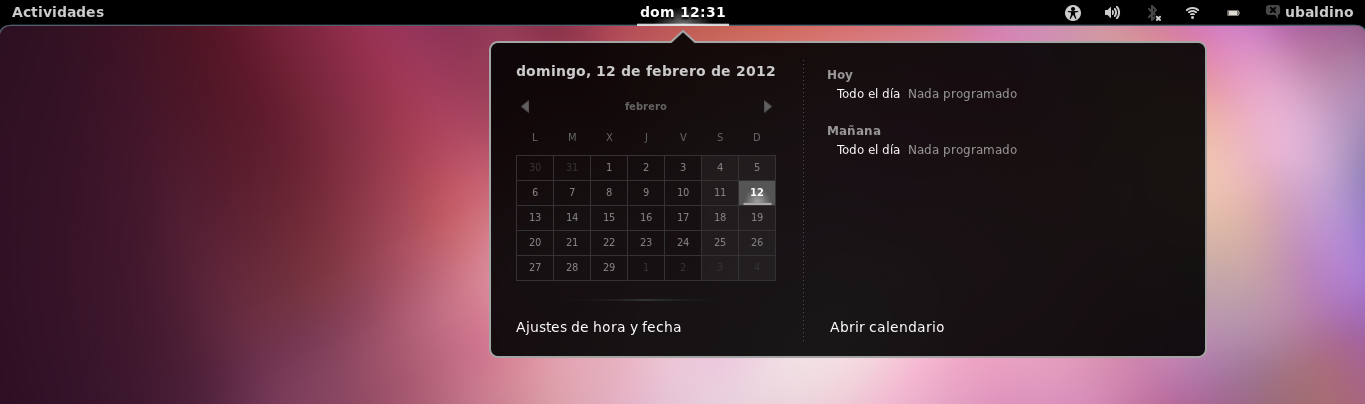
\includegraphics[scale=0.448]{gnome/barra.png}
\end{center}
Gnome es uno de los tantos escritorios que existen para las distribuciones basadas en linux.
En este caso UBUNTU 11.10 utiliza el escritorio o interfaz gráfica Gnome 3, y como es de esperar de un escritorio, los componentes principales del escritorio Gnome son:
\begin{itemize}
\item[-] Iconos que enlazan a archivos, carpetas o programas (accesos directos).
\item[-] Gnome Shell que es la barra de tareas y lanzador de aplicaciones. y tiene un gestor de ventanas con soporte OpenGL.
\begin{description}
\item[Gnome Shell] tiene un panel único en la parte superior, que contiene:
\begin{itemize}
 \item menú de usuario. 
 \item un botón “actividades”. 
 \item aplicaciones en ejecución.
 \item reloj.
 \item área de accesibilidad.
 \item control de volumen.
 \item información de la red.
 \item estado de la batería en el caso de un portátil.
\end{itemize}
En el arranque del sistema aparece dicho panel y el fondo de escritorio.
\end{description}
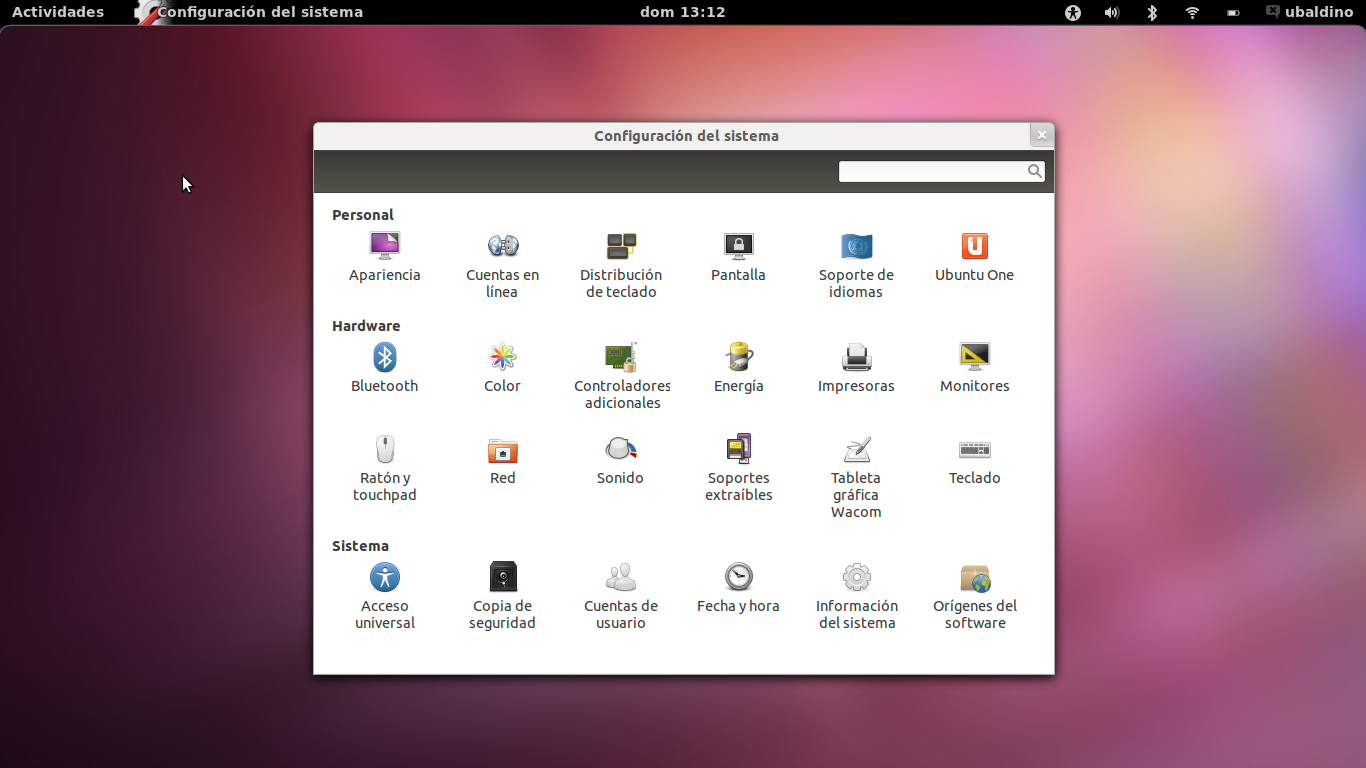
\includegraphics[scale=0.35]{gnome/Pantallazo3.png}\\ 
Al pulsar sobre “actividades” o acercar el ratón con rapidez a la esquina superior izquierda, se despliegan varios elementos nuevos:
\begin{itemize}
\item A la izquierda, un panel lanzador de aplicaciones,
\item Bajo el panel superior, un menú de dos opciones, “ventanas” y “aplicaciones”.
\item A la derecha, otro panel con una vista previa de las ventanas activas que actúa como selector de escritorios y por encima de éste, una caja de búsqueda.
\end{itemize}
Si tienes ya algún programa en ejecución, que por defecto se lanza a pantalla completa, la ventana o ventanas activas que su reducen su tamaño mostrando una leyenda informativa en la parte inferior de cada ventana. Cada acción que comporte cambios de tamaño o posición, vendrá acompañada de una elegante animación y otros efectos visuales.\\
El botón gráfico windows (ventanas), restaura la vista previa de aquellas que estén activas si las has perdido de vista por ejecutar cualquier otra acción.\\
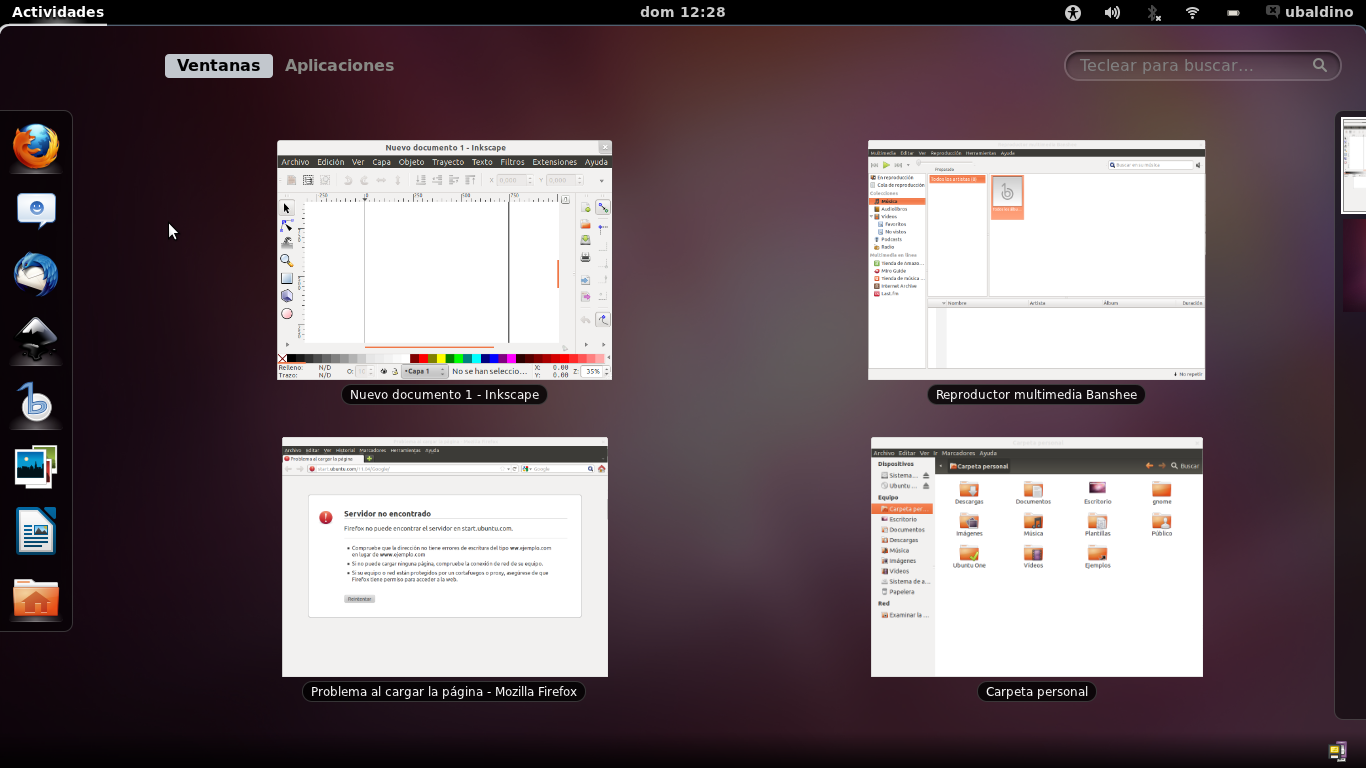
\includegraphics[scale=0.35]{gnome/Pantallazo4.png}\\ 

El botón aplications (aplicaciones), da paso a la representación mediante iconos de los programas instalados en la máquina.\\

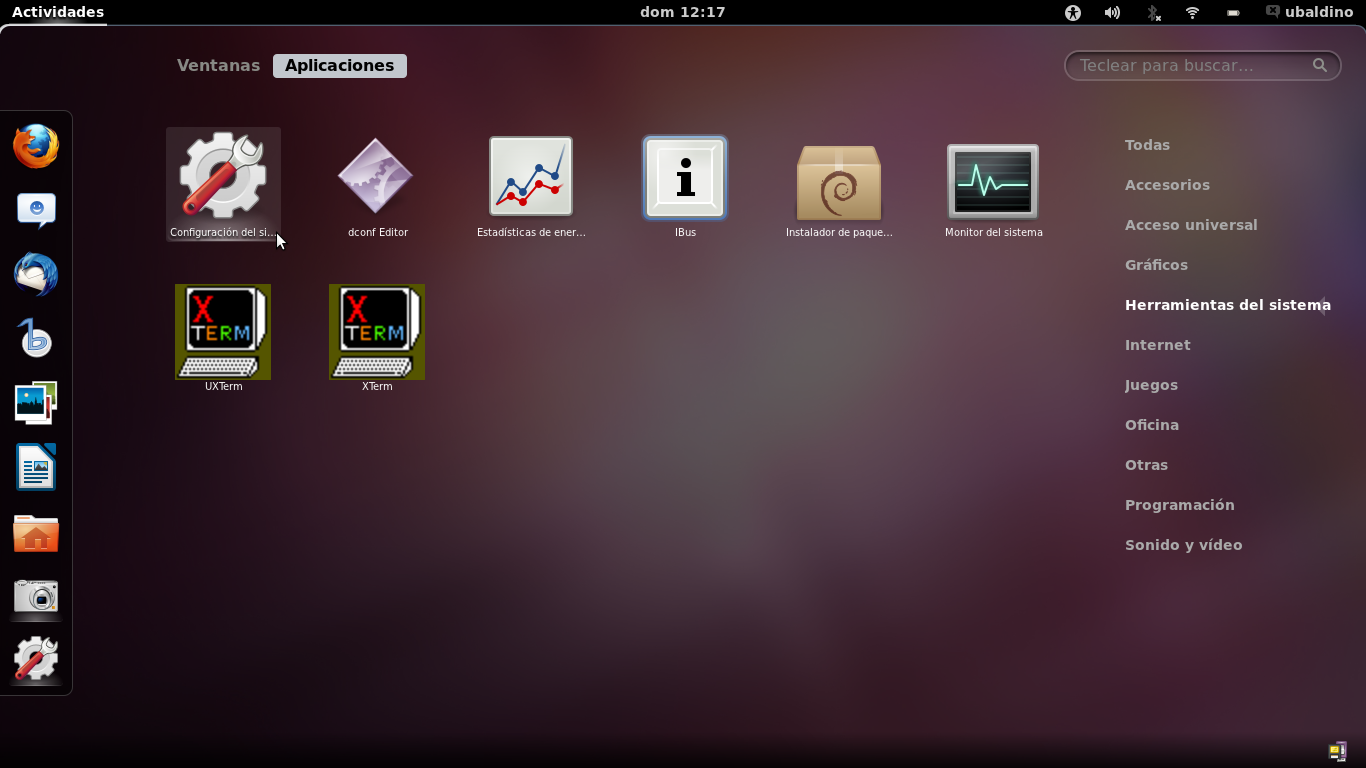
\includegraphics[scale=0.35]{gnome/Pantallazo5.png} \\
\underline{\bf Nota:} Note que cuando estamos en la presentación de los programas instalados en la maquina. El panel de la derecha porta un sistema de filtrado, clasificando los programas según las funcionalidades.\\

La caja de búsqueda es lo novedoso de gnome 3. Escribiendo las primeras letras de una aplicación, aparecerá de forma inmediata el icono correspondiente al programa y puedes lanzar la aplicación desde ahí. Y en la parte inferior de la pantalla muestra dos botones gráficos, que permiten extender la búsqueda en Wikipedia y Google.\\ 

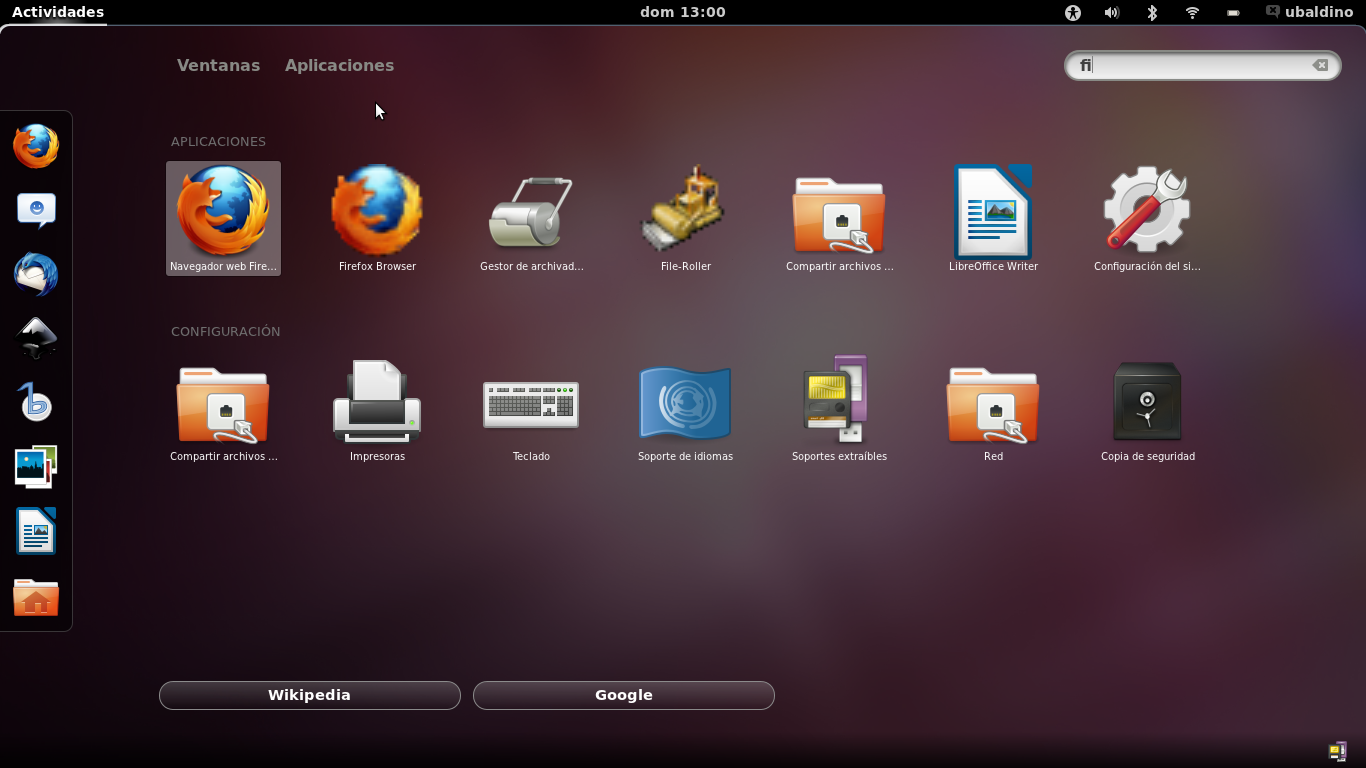
\includegraphics[scale=0.35]{gnome/Pantallazo6.png}\\ 

Por último, terminando nuestro recorrido en Gnome Shell, en la parte inferior derecha de la pantalla veremos el área de notificaciones y bandeja de mensajes, desde donde puedes contestar con el programa de mensajería instantánea.\\
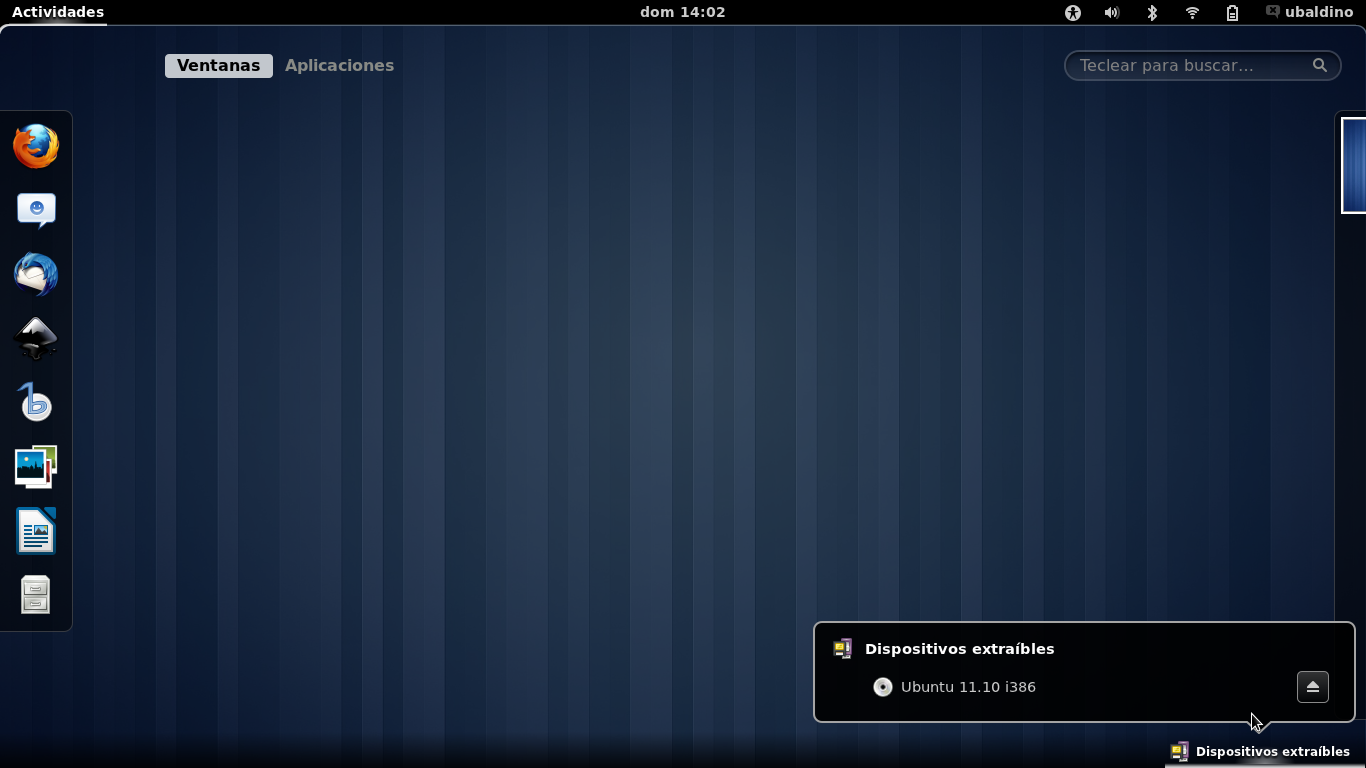
\includegraphics[scale=0.35]{gnome/Pantallazo7.png} 
\end{itemize}
\section{Ventanas y áreas de trabajo}
Como otros escritorios, GNOME usa ventanas para mostrar las aplicaciones en ejecución. Usando la vista y el tablero, puede lanzar aplicaciones nuevas y controlar qué ventana está activa.\\

Además de en las ventanas, también puede agrupar sus aplicaciones en áreas de trabajo. Visite los temas de ayuda de ventana y área de trabajo que se muestran a continuación para aprender mejor cómo usar estas características.

\subsection{Trabajar con ventanas}
\subsubsection{Cambiar entre ventanas}
\subsubsection{Encontrar una ventana perdida}
\subsubsection{Maximizar y des-maximizar (restaurar) una ventana}
\subsubsection{Operaciones de ventanas}
\subsubsection{Ventanas en mosaico}

\subsection{Trabajar con áreas de trabajo}
\subsubsection{¿Que es un área de trabajo y cómo me ayudará?}
\subsubsection{Cambie entre las áreas de trabajo}
\subsubsection{Mover una ventana a un área de trabajo diferente}
